% Copyright 2004 by Till Tantau <tantau@users.sourceforge.net>.
%
% In principle, this file can be redistributed and/or modified under
% the terms of the GNU Public License, version 2.
%
% However, this file is supposed to be a template to be modified
% for your own needs. For this reason, if you use this file as a
% template and not specifically distribute it as part of a another
% package/program, I grant the extra permission to freely copy and
% modify this file as you see fit and even to delete this copyright
% notice. 

\documentclass[xcolor=dvipsnames]{beamer}
\usepackage{bibentry}
\setbeamertemplate{bibliography item}{\insertbiblabel}
\usepackage{cancel}
\usepackage{amsmath} 
\usepackage{mathtools}
\newcommand{\norm}[1]{\left\lVert #1 \right\rVert}
% Command for round parenthesis
\newcommand{\roundP}[1]{\left( #1 \right)}
% Command for poisson brackets
\newcommand{\poisson}[2]{\left\lbrace #1, #2 \right\rbrace}

\usepackage{varwidth}
\usepackage{lipsum}
\usepackage{color}
\usepackage{todonotes}
\definecolor{dgray}{gray}{0.30}
\definecolor{uyellow}{RGB}{253,241,0}

\usepackage[utf8]{inputenc}
\usepackage{graphicx}
\usepackage{epstopdf}
\usepackage[english]{babel}
\usepackage{hyperref}
\usepackage{datenumber}
\usepackage{todonotes}
\usepackage{mathtools}
\usepackage{amsmath}
\usepackage{amssymb}
\usepackage{amsthm}

\newtheorem*{thm}{Theorem}
\newcommand{\fmunu}{F^{\mu\nu}}
\newcommand{\E}{\vec{E}}
\newcommand{\B}{\vec{B}}
\newcommand{\rot}{\nabla\times}
\newcommand{\dive}{\nabla\cdot}
\newcommand{\tmunu}{T^{\mu\nu}}
\newcommand{\levichi}{\epsilon_{\mu\nu\sigma\gamma}}
\newcommand{\dete}{\textrm{det}}
\newcommand{\lna}{\textrm{ln}}
\newcommand{\Tr}{\textrm{Tr}}
\newcommand{\seno}{\textrm{sin}}

\makeatletter
\newcommand{\pushright}[1]{\ifmeasuring@#1\else\omit\hfill$\displaystyle#1$\fi\ignorespaces}
\newcommand{\pushleft}[1]{\ifmeasuring@#1\else\omit$\displaystyle#1$\hfill\fi\ignorespaces}
\makeatother



% There are many different themes available for Beamer. A comprehensive list with examples is given here:
% http://deic.uab.es/~iblanes/beamer_gallery/index_by_theme.html
%\usetheme{AnnArbor}
%\usetheme{Antibes}
%\usetheme{Bergen}
%\usetheme{Berkeley}
%\usetheme{Berlin}
%\usetheme{Boadilla}
%\usetheme{boxes}
%\usetheme{CambridgeUS}
\usetheme{Copenhagen}
%\usetheme{Darmstadt}
%\usetheme{default}
%\usetheme{Frankfurt}
%\usetheme{Goettingen}
%\usetheme{Hannover}
%\usetheme{Ilmenau}
%\usetheme{JuanLesPins}
%\usetheme{Luebeck}
%\usetheme{Madrid}
%\usetheme{Malmoe}
%\usetheme{Marburg}
%\usetheme{Montpellier}
%\usetheme{PaloAlto}
%\usetheme{Pittsburgh}
%\usetheme{Rochester}
%\usetheme{Singapore}
%\usetheme{Szeged}
%\usetheme{Warsaw}
%\usecolortheme{seagull}
%\usetheme{Malmoe} 
\usepackage{graphicx,caption}
\setbeamercolor{frametitle}{fg=Black,bg=Blue!60}
\setbeamercolor{section in head/foot}{bg=Blue, fg=Black}
\setbeamercolor{author in head/foot}{bg=blue, fg=Black} 
\setbeamercolor{date in head/foot}{fg=blue} 
\setbeamercolor{institute in head/foot}{fg=Black}
\usecolortheme[named=Black]{structure}
\setbeamerfont{footnote}{size=\footnotesize}

\setbeamertemplate{}[page number] % To replace the footer line in all slides with a simple slide count uncomment this line
 
\title{\textbf{Environmental dependence of HI-Mass functions in cosmological simulations}}

% A subtitle is optional and this may be deleted
%\subtitle{Optional Subtitle}

\author{Jesus Prada}
% - Give the names in the same order as the appear in the paper.
% - Use the \inst{?} command only if the authors have different affiliation.

\institute[{\color{Black} Universidad de los Andes}] % (optional, but mostly needed)
{
Advisor: PhD Jaime Forero-Romero\\
Universidad de los Andes, Physics Department\\
In collaboration with:\\
PhD Michael Jones - Cornell University\\
PhD Martha Haynes - Cornell University \\
}
% - Use the \inst command only if there are several affiliations.
% - Keep it simple, no one is interested in your street address.

\tiny
\date{ \footnotesize October, 2016}
% - Either use conference name or its abbreviation.
% - Not really informative to the audience, more for people (including yourself) who are reading the slides online
	

\subject{The effect of environment on HI-mass functions in cosmological simulations}
% This is only inserted into the PDF information catalog. Can be left out. 

% If you have a file called "university-logo-filename.xxx", where xxx  is a graphic format that can be processed by latex or pdflatex, resp., then you can add a logo as follows:
% \pgfdeclareimage[height=0.5cm]{university-logo}{university-logo-filename}
% \logo{\pgfuseimage{university-logo}}

% Delete this, if you do not want the table of contents to pop up at the beginning of each subsection:
%\AtBeginSubsection[] { \begin{frame}<beamer>{Outline} \tableofcontents[currentsection,currentsubsection] \end{frame}}

% Let's get started
\begin{document}

\begin{frame}
  \titlepage
\end{frame}
%--------------------------------------------
\begin{frame}{Outline}
 \tableofcontents
  % You might wish to add the option [pausesections]
\end{frame}
%------------------------------------------------
\section{Introduction}
\subsection{Mass functions and Press-Schechter formalism}
\begin{frame}
\begin{itemize}
\small
\item Histogram of masses of galaxies and halos
\item Logarithmic scales are needed for better interpretation
\item Press-Schechter adjusts surprisingly well to observations
\end{itemize}
$$n(M) = \phi_* \left( \frac{M}{M_*}\right)^{\alpha+1}e^{\left( \frac{M}{M_*}\right)}$$
\normalsize
\begin{figure}[h!]
\centering
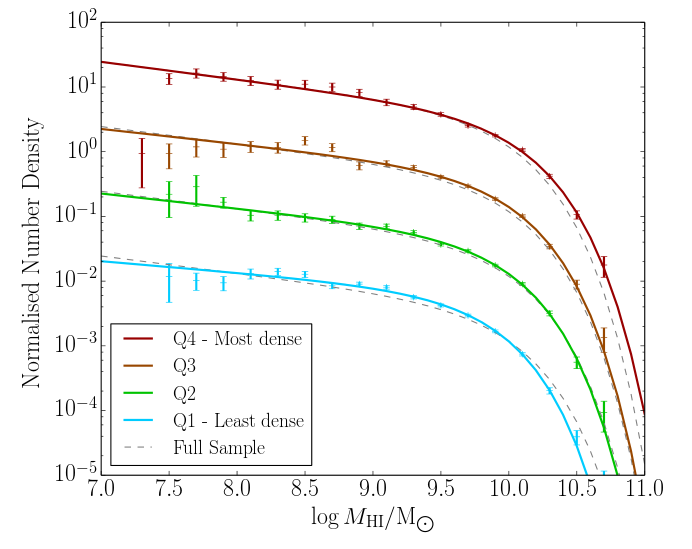
\includegraphics[width=0.55\textwidth]{schechterFits}
\centering
{\tiny \\ Jones et al. \cite{jones}}
\end{figure}
\end{frame}
%--------------------------------------------------------------------------------------
\subsection{Environment}
\begin{frame}
\begin{itemize}
\item Related to the mass density 
\item Useful to verify its effect on the physics of galaxy formation
\item Great variety of methods to quantify environment
\item Nearest neighbour, control volume \cite{environments}.  
\item 3rd Nearest neighbour (Observational) \cite{jones}
\item T-Web structures (Theoretical) Forero-Romero et al. \cite{forero}
\end{itemize}
\end{frame}
%-----------------------------------------------------------------------------------------
\subsection{3rd Nearest neighbour method}
\begin{frame}
\begin{itemize}
\item Projected distance on sky.
\item Velocity cut is needed.
\item Distance to 3rd (not 1st) neighbour is required to avoid noise.
\end{itemize}
\begin{figure}[h!]
\centering
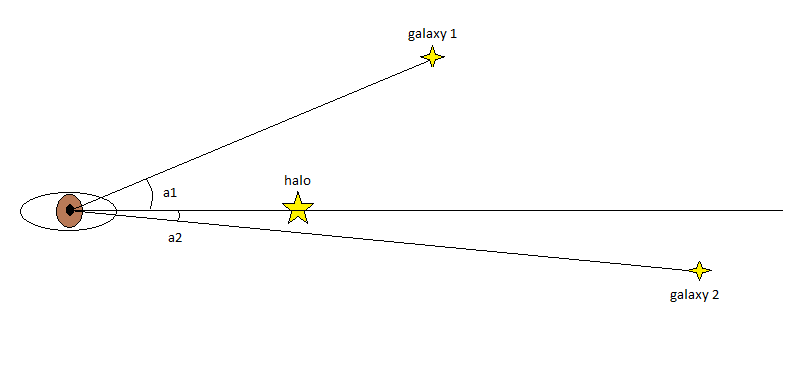
\includegraphics[width=0.7\textwidth]{nearest_neighbor}
\centering
\end{figure}
\end{frame}
%---------------------------------------------------------------------------------------
\subsection{T-Web structures}
\begin{frame}
\begin{itemize}
\item Hessian of gravitational potential.
\item 3 eigenvalues can identify 4 structures
\item Clusters, sheets, filaments and voids.
\end{itemize}
\begin{figure}[ht]
        \begin{minipage}[b]{0.45\linewidth}
            \centering
            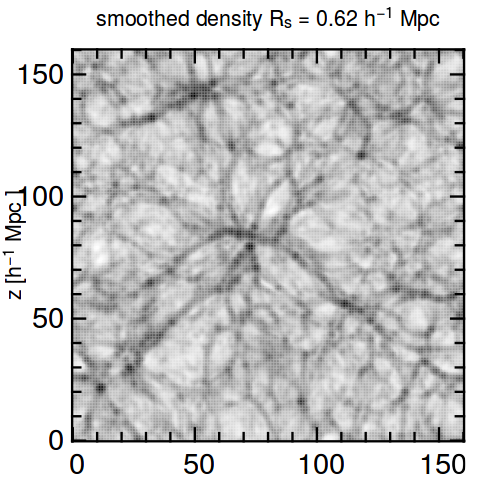
\includegraphics[width=\textwidth]{tweb}
            {\tiny \ \ \ \ \   Forero-Romero et al. \cite{forero}}

        \end{minipage}
        \hspace{0.5cm}
        \begin{minipage}[b]{0.45\linewidth}
            \centering
            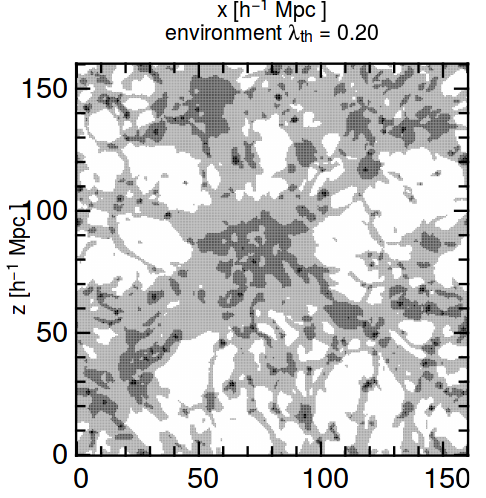
\includegraphics[width=\textwidth]{tweb2}
            {\tiny \ \ \ \ \ Forero-Romero et al. \cite{jones}}
        \end{minipage}
    \end{figure}
\end{frame}
%-------------------------------------------------------------------------
\section{Motivation}
\begin{frame}
\begin{itemize}
\item HIPASS and ALFALFA big surveys allow the study of HI-Mass functions.
\item The effect of environment on the physics of galaxy formation.
\item Mass tendency to cluster.
\item Voids: slow evolution. Sample HIMF at earlier times.
\item Studies are so recent and sometimes contradict each others (Springob, Haynes \& Giovanelli) \cite{contra1} and Stierwalt et al. \cite{contra2}.
\end{itemize}
\end{frame}
%---------------------------------------------------------------------------
%-------------------------------------------------------------------------
\begin{frame}
\section{Our Work}
\subsection{Illustris run}

\begin{figure}[ht]
        \begin{minipage}[b]{0.5\linewidth}
            \begin{itemize}
			\item Illustris run
			\item $106.5Mpc$
			\item $1820^3$ particles
			\item $6.3\cdot 10^{6}M_{\odot}$ DM resolution
			\item $1.3\cdot 10^{6}M_{\odot}$ Gas resolution
			\item Detailed galaxy characteristics
			\end{itemize}

        \end{minipage}
        \hspace{0.0cm}
        \begin{minipage}[b]{0.40\linewidth}
            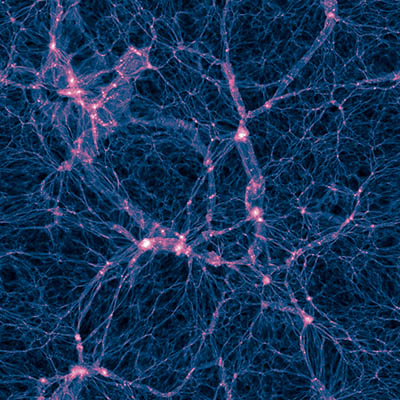
\includegraphics[width=1\textwidth]{illustris}
			\centering
			{\tiny \ \ \ \ \ http://www.illustris-project.org/media/}
        \end{minipage}
    \end{figure}

\end{frame}
%---------------------------------------------------------------------------
\subsection{Results}
\begin{frame}
\begin{itemize}
			\item Distance to 3rd nearest neighbour for galaxies with gas.
			\item Divided group in quartiles and obtained Schechter fits.
\end{itemize}
\begin{figure}[h!]
\centering
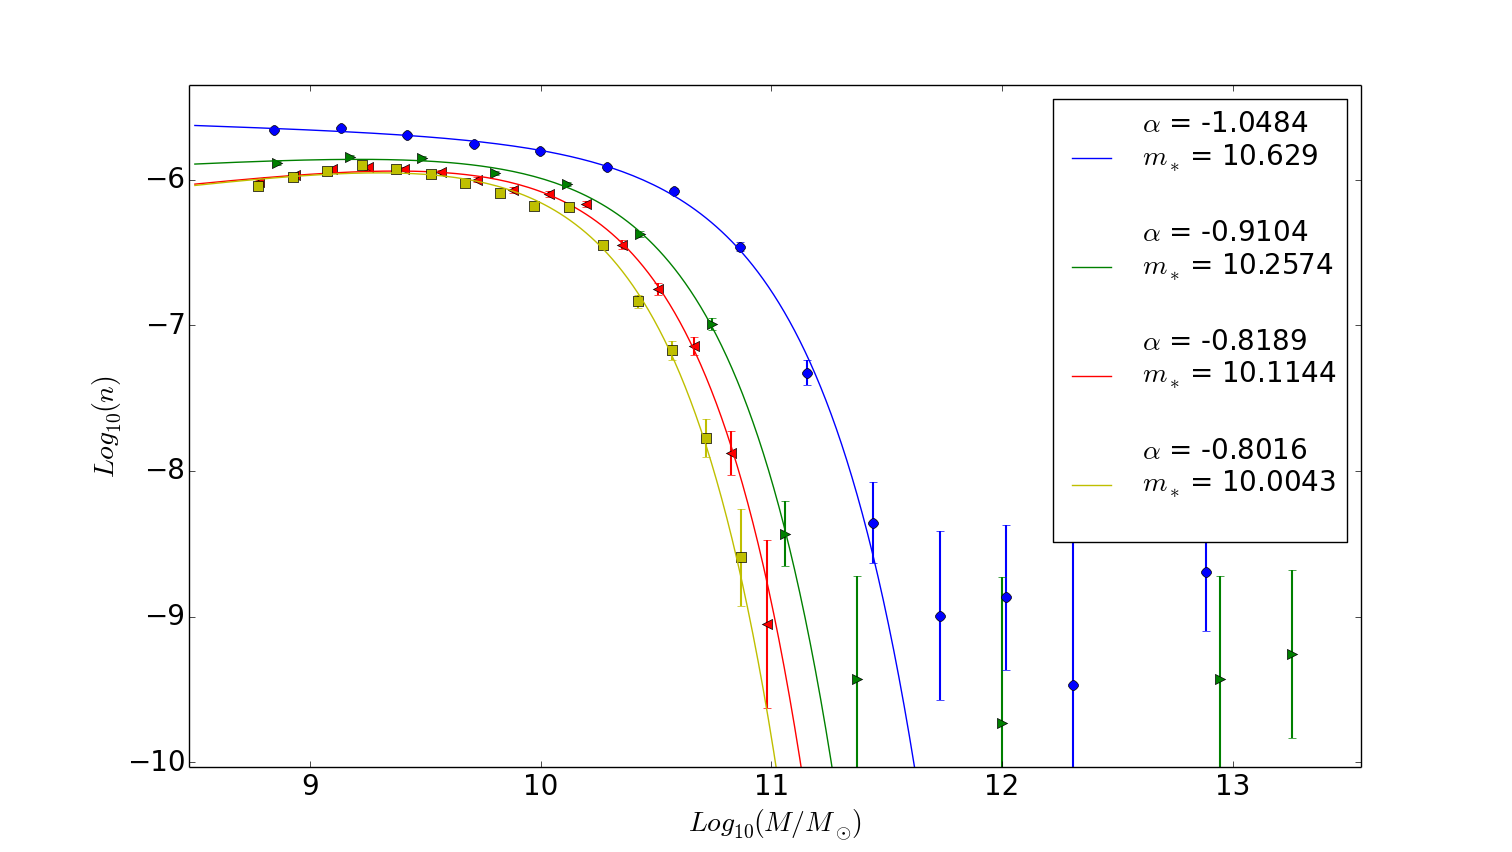
\includegraphics[width=0.9\textwidth]{environment1}
\centering
\end{figure}
\end{frame}
%---------------------------------------------------------------------------
\begin{frame}
\begin{figure}[h!]
        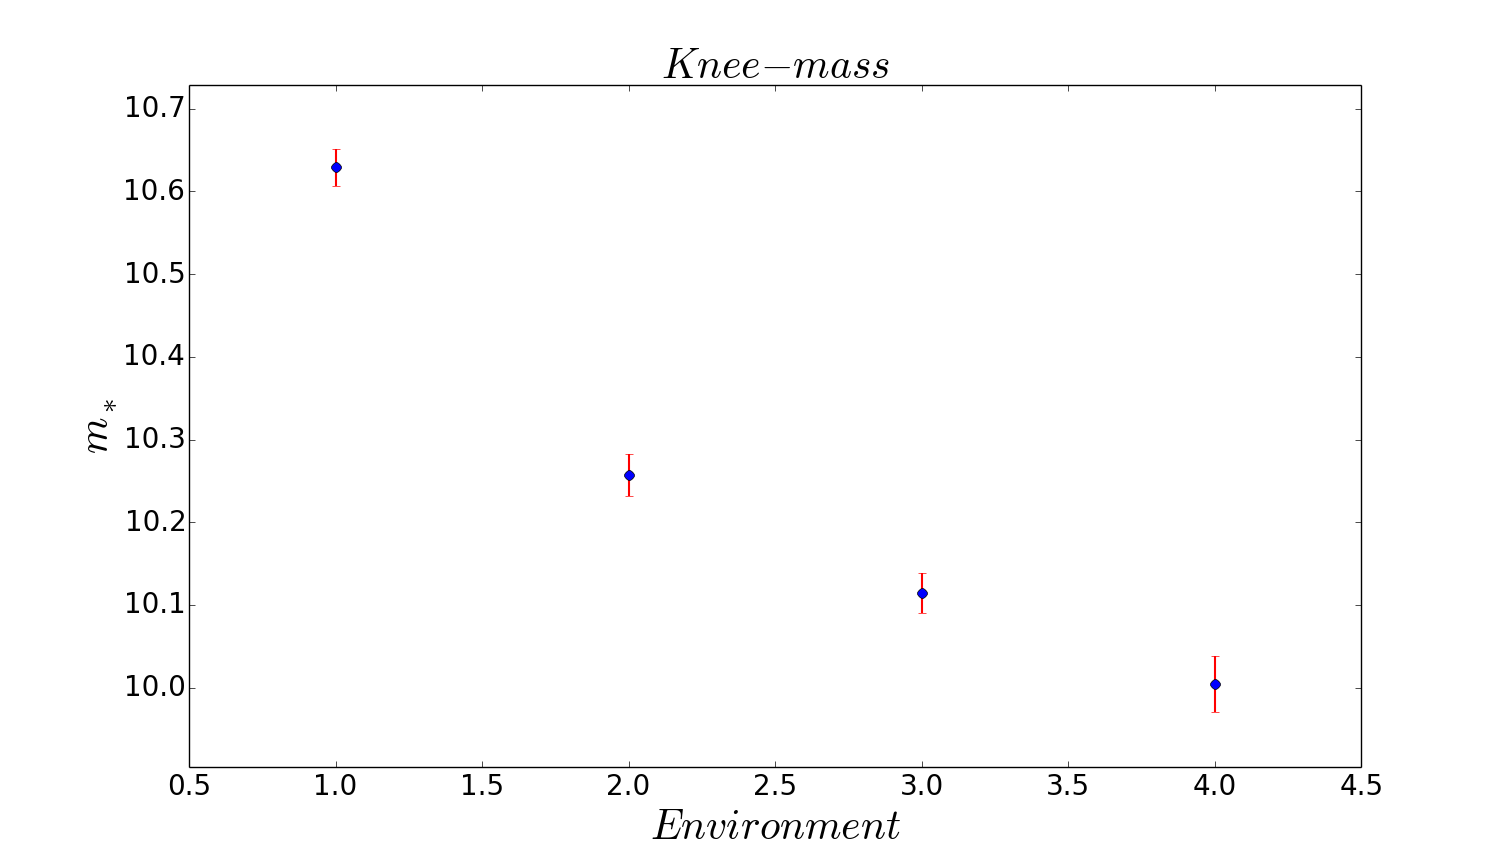
\includegraphics[width=0.55\textwidth]{m1}
\end{figure}
\begin{figure}[h!]
	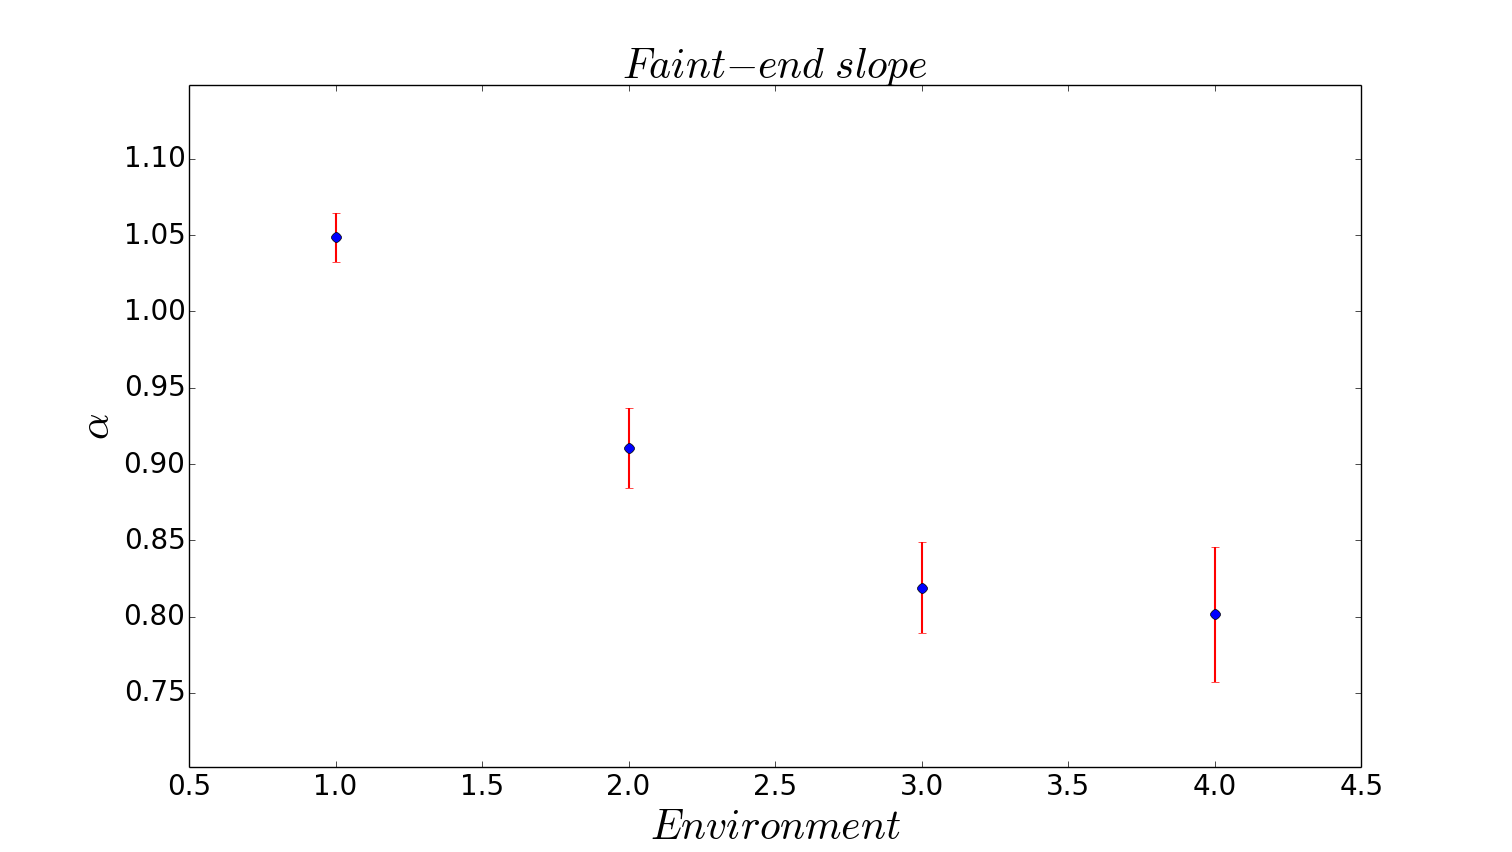
\includegraphics[width=0.55\textwidth]{alpha1}
\end{figure}
\end{frame}
%---------------------------------------------------------------------------
\begin{frame}
\begin{itemize}
			\item Divided galaxies into Cluster,Sheet,filament and void groups.
			\item Obtained Schechter fits.
\end{itemize}
\begin{figure}[h!]
\centering
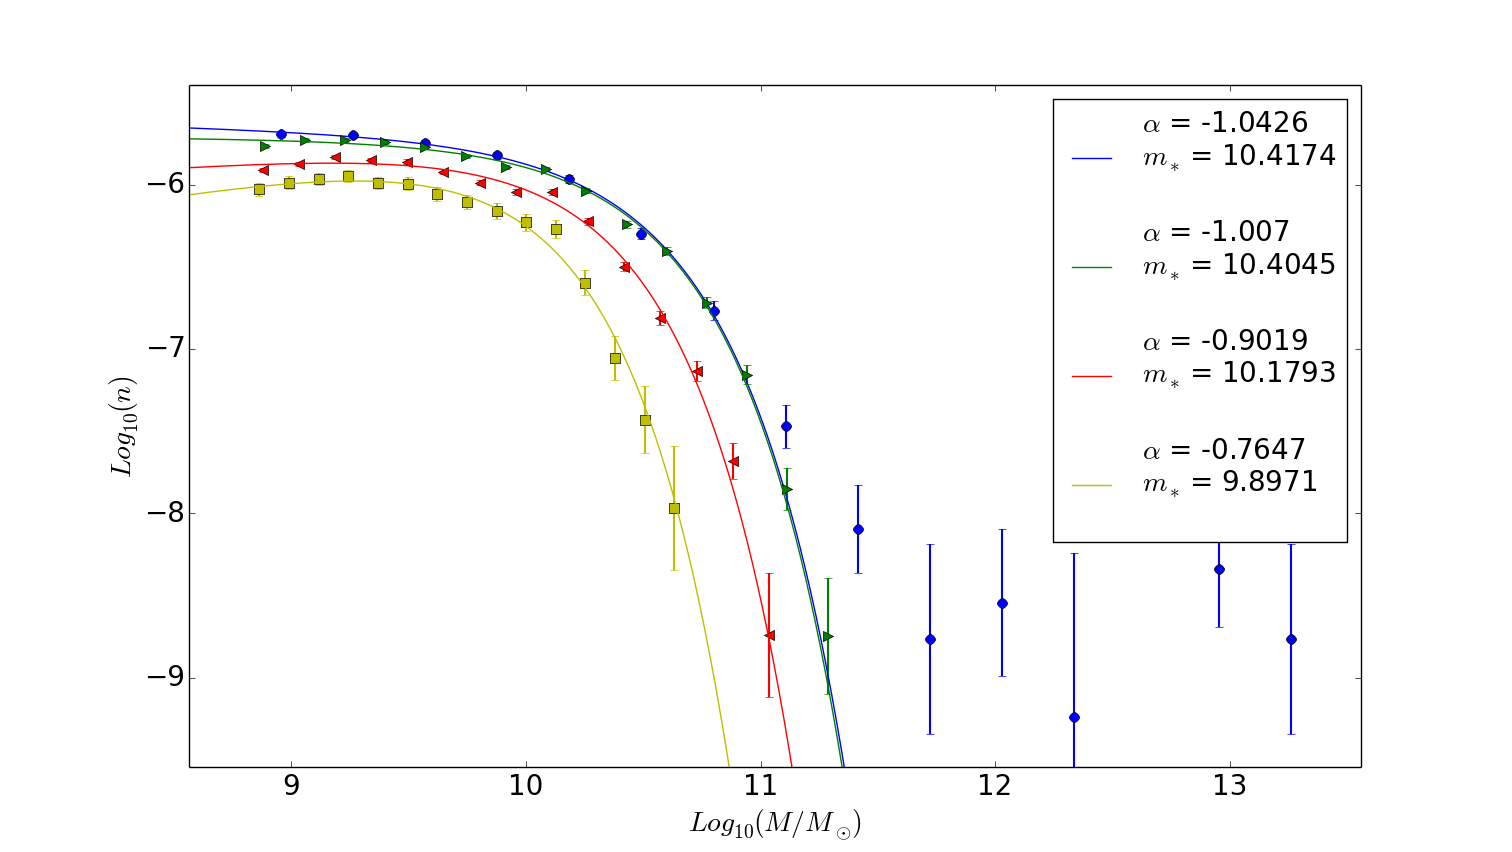
\includegraphics[width=0.9\textwidth]{environment2}
\centering
\end{figure}
\end{frame}

\begin{frame}
\begin{figure}[h!]
        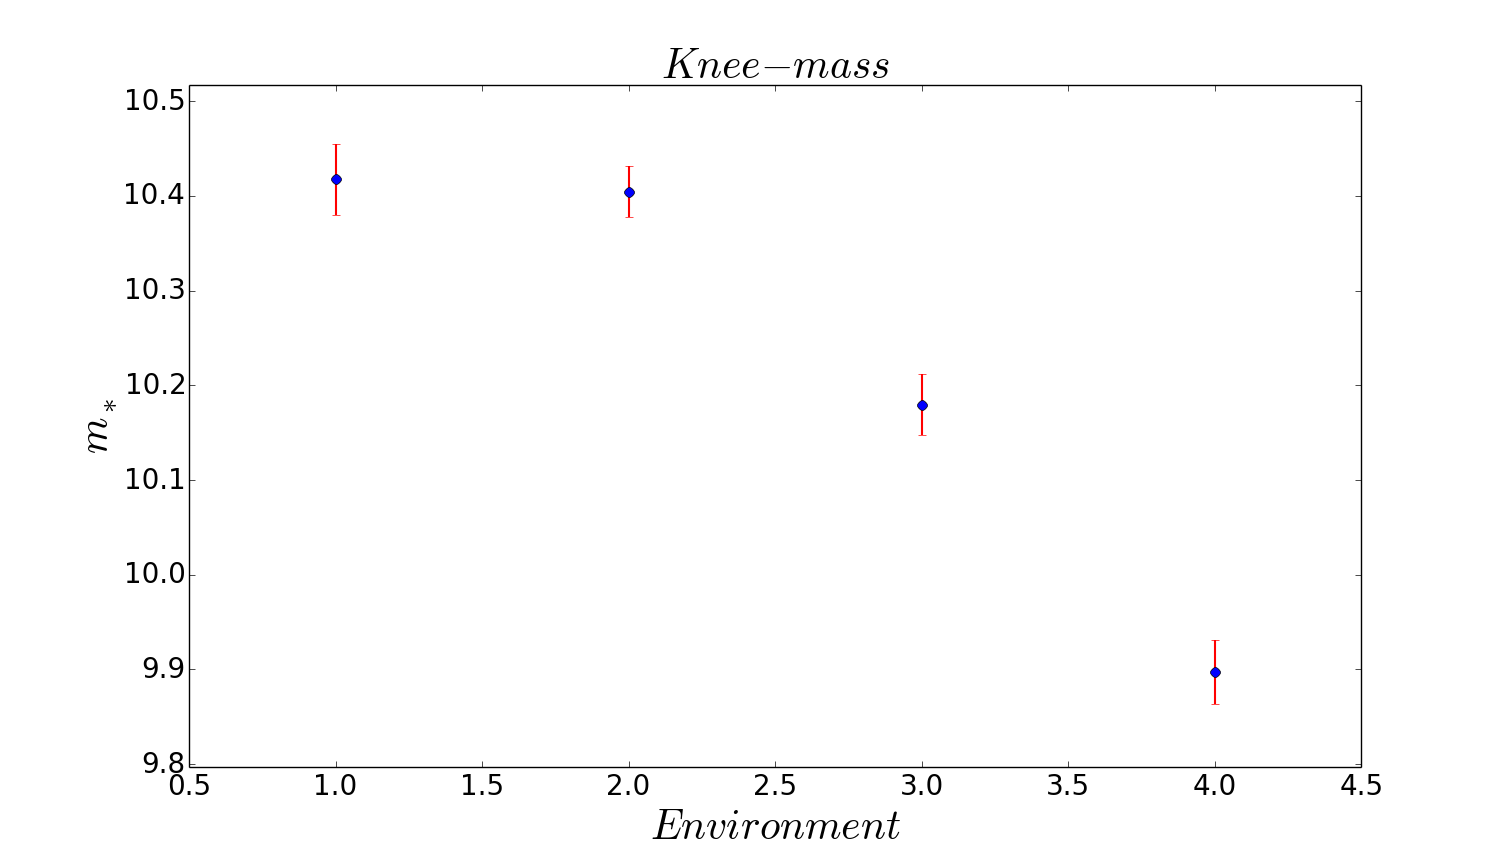
\includegraphics[width=0.55\textwidth]{m2}
\end{figure}
\begin{figure}[h!]
	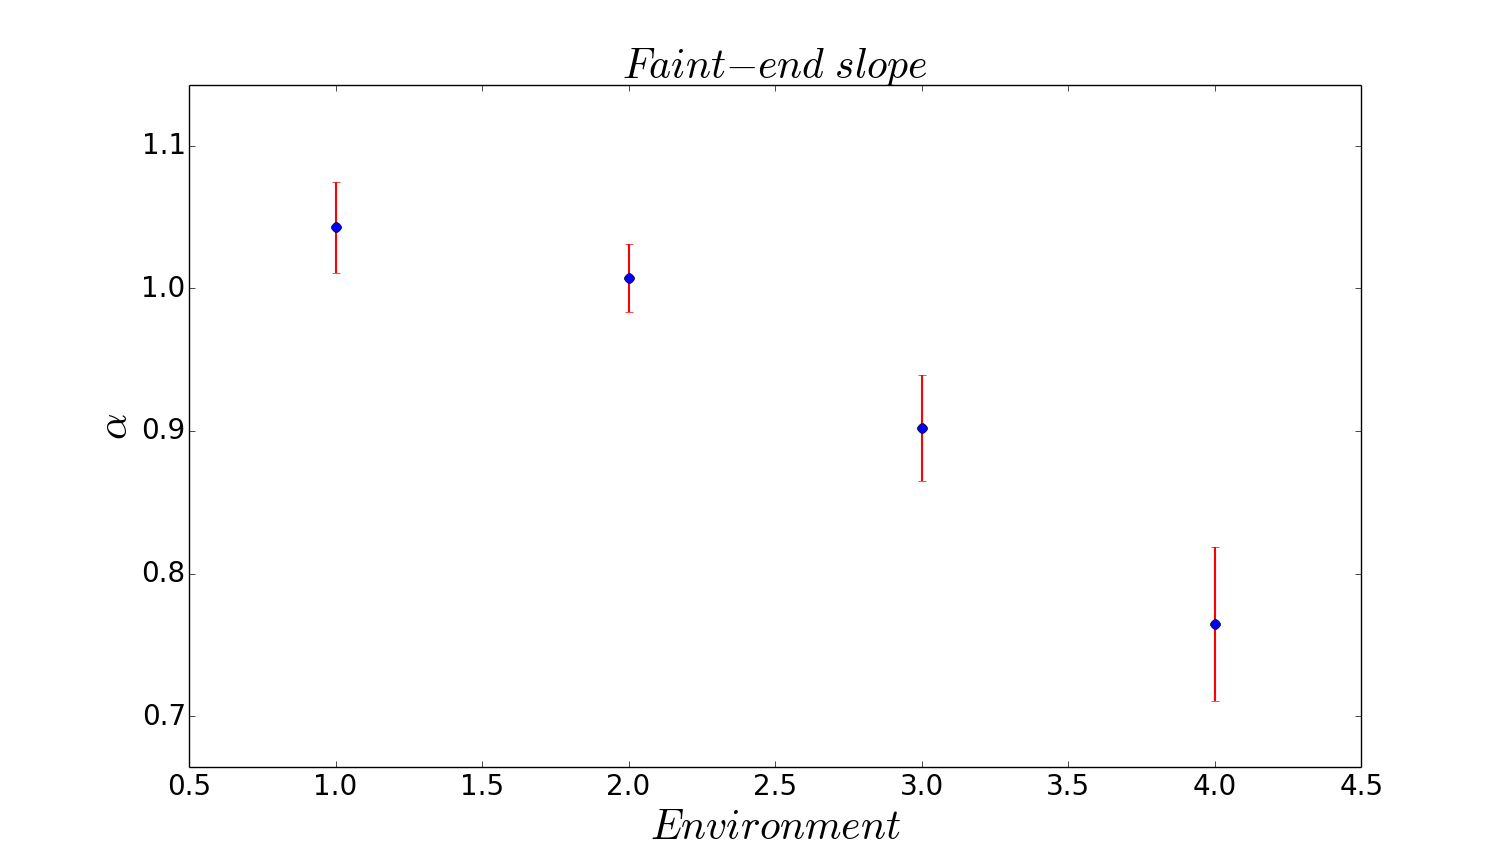
\includegraphics[width=0.55\textwidth]{alpha2}
\end{figure}
\end{frame}
%---------------------------------------------------------------------------
\subsection{Conclusions}
\begin{frame}
\begin{itemize}
			\item We obtained a clear general tendency for the knee-mass and the faint-end slope in both methods.
			\item For high density environments from T-web, both tendencies becomes more diffuse.
			\item For low density neighbouring environments, the faint-end slope relation is diffuse. 
\end{itemize}
\end{frame}
\begin{frame}
\begin{itemize}
			\item The knee-mass increases with neighbouring density in a range from $10.00\pm0.03$ to $10.62\pm0.02$.
			\item For Cosmic web environment the range is from $9.90\pm0.03$ to $10.41\pm0.04$.
			\item Faint-end ranges are $[-0.80\pm0.04,-1.05\pm0.02]$ and $[-0.76\pm0.05,1.04\pm0.03]$.
\end{itemize}
\end{frame}
%---------------------------------------------------------------------------
\subsection{Further Work}
\begin{frame}
\begin{itemize}
			\item Detailed analysis of effects for big-scale environments using both methods.
			\item Relation between of different mass functions (DM-SMBH-gas).
			\item Incorporate a reasonable approximation for HI mass in terms of gas mass.
\end{itemize}
\end{frame}


\section{References}
\begin{frame}[t, allowframebreaks]
\frametitle{Referencias}
\tiny
\bibliographystyle{unsrt}
\bibliography{Bibliography}
\end{frame}
\end{document}
